% template.tex
% Toyohashi Tech Beamer slide template
% Build: latexmk -lualatex template.tex
% Fallback: lualatex -interaction=nonstopmode template.tex
% (If using minted instead of listings, add -shell-escape)
\documentclass[aspectratio=169,unicode]{beamer}

% ========== Font: LuaLaTeX + luatexja ==========
\usepackage{luatexja}
\usepackage[haranoaji]{luatexja-preset}
\usepackage{fontspec}
% Prefer Hiragino on macOS; fall back to HaranoAji set above otherwise.
\IfFontExistsTF{HiraKakuProN-W3}{%
  \setmainjfont[BoldFont={HiraKakuProN-W6}]{HiraKakuProN-W3}%
}{}

% ========== Packages ==========
\usepackage{amsmath, amssymb}
\usepackage{tikz}
\usetikzlibrary{arrows.meta, positioning, shapes.geometric}
\usepackage[ruled,vlined]{algorithm2e}
\usepackage{listings}   % Or: \usepackage{minted} (requires latexmk -lualatex -shell-escape)
\usepackage{tcolorbox}
\usepackage{graphicx}
\usepackage{etoolbox}

% ========== Toyohashi Tech theme ==========
\usetheme{Toyohashi}
\graphicspath{{images/}}

% ========== listings settings ==========
\lstset{
  basicstyle=\ttfamily\small,
  frame=single,
  backgroundcolor=\color{black!5},
  breaklines=true,
  showstringspaces=false,
  keywordstyle=\color{tutred}\bfseries,
  commentstyle=\color{black!60}\itshape,
}

% ========== Document metadata ==========
\title{スライドタイトル}
\subtitle{サブタイトル（任意）}
\author{発表者名}
\date{\today}

\begin{document}

% ============================================================
% 1) Title slide (plain: hide footer decorations)
% ============================================================
\begin{frame}[plain,noframenumbering]
  \titlepage
\end{frame}

% ============================================================
% 2) 篇首タイトル + bullet + tuthighlight ボックス + 下向き矢印
% ============================================================
\begin{frame}{篇首タイトル}
  \begin{itemize}
    \item イーハトーヴのすきとおった風、夏でも底に冷たさをもつ青いそら
    \item うつくしい森で飾られたモリーオ市、郊外のぎらぎら光る草の波
  \end{itemize}
  \vspace{0.4em}
  \begin{center}
    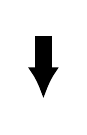
\begin{tikzpicture}
      \draw[-{Latex[length=4mm,width=4mm]}, line width=6pt, black]
        (0,0.4) -- (0,-0.4);
    \end{tikzpicture}
  \end{center}
  \begin{tuthighlight}
    ここに結論となる強調文を入れる
  \end{tuthighlight}
\end{frame}

% ============================================================
% 3) 2カラム比較 (小タイトル×2 + 各 bullet)
% ============================================================
\begin{frame}{2カラム比較}
  \begin{columns}[T]
    \begin{column}{0.48\textwidth}
      \begin{center}\textbf{左タイトル}\end{center}
      \begin{itemize}
        \item よだかは、実にみにくい鳥です
        \item 顔は、ところどころ、味噌をつけたようにまだらです
        \item くちばしは、ひらたくて、耳までさけています
      \end{itemize}
    \end{column}
    \begin{column}{0.48\textwidth}
      \begin{center}\textbf{右タイトル}\end{center}
      \begin{itemize}
        \item 足はまるでよぼよぼで、一間とも歩けません
        \item 他の鳥は、よだかの顔を見ただけでも、いやになってしまう
      \end{itemize}
    \end{column}
  \end{columns}
\end{frame}

% ============================================================
% 4) 両カラム図パターン
% ============================================================
\begin{frame}{両カラム図パターン}
  \begin{columns}[T]
    \begin{column}{0.48\textwidth}
      \begin{center}
        \begin{tikzpicture}
          \node[draw, rounded corners, minimum width=4cm, minimum height=2.8cm,
                fill=tutred!12] {図（左）};
        \end{tikzpicture}
      \end{center}
    \end{column}
    \begin{column}{0.48\textwidth}
      \begin{center}
        \begin{tikzpicture}
          \node[draw, rounded corners, minimum width=4cm, minimum height=2.8cm,
                fill=black!8] {図（右）};
        \end{tikzpicture}
      \end{center}
    \end{column}
  \end{columns}
\end{frame}

% ============================================================
% 5) 左説明 / 右図パターン
% ============================================================
\begin{frame}{左説明 / 右図パターン}
  \begin{columns}[T]
    \begin{column}{0.5\textwidth}
      \begin{itemize}
        \item ざしき童子（ぼっこ）というのは、
        \item このような子供のことをいうのです
        \item いかにも、うるさく、そうぞうしくして、
        \item ざしきわらしのやうに聞けている
      \end{itemize}
    \end{column}
    \begin{column}{0.48\textwidth}
      \begin{center}
        \begin{tikzpicture}
          \node[draw, rounded corners, minimum width=4cm, minimum height=3.4cm,
                fill=tutred!10] {図};
        \end{tikzpicture}
      \end{center}
    \end{column}
  \end{columns}
\end{frame}

% ============================================================
% 6) 横広×縦小の図は下配置（タイトルとの干渉回避）
% ============================================================
\begin{frame}{横広×縦小の図は下配置}
  \begin{itemize}
    \item 横に広く縦が短い図（横長グラフ・タイムラインなど）は
    \item スライドタイトル・二重線との干渉を避けるため下側に配置する
  \end{itemize}
  \vfill
  \begin{center}
    \begin{tikzpicture}
      \node[draw, rounded corners, minimum width=11cm, minimum height=1.8cm,
            fill=tutred!8]
        {横広×縦小の図（例：タイムライン）};
    \end{tikzpicture}
  \end{center}
  \vspace{0.4em}
\end{frame}

% ============================================================
% 7) 数式スライド
% ============================================================
\begin{frame}{数式スライド}
  \begin{align}
    \mathcal{L}(\theta) &= -\sum_{i=1}^{N} \log p_\theta(y_i \mid x_i) \\
    \nabla_\theta \mathcal{L} &= -\sum_{i=1}^{N} \nabla_\theta \log p_\theta(y_i \mid x_i)
  \end{align}
  \vspace{0.2em}
  \begin{tuthighlight}
    強調したい結論をハイライトボックスに入れる
  \end{tuthighlight}
\end{frame}

% ============================================================
% 8) tikz 図の例
% ============================================================
\begin{frame}{tikz 図の例}
  \begin{center}
    \begin{tikzpicture}[
        node distance=1.8cm,
        every node/.style={draw, rounded corners,
                          minimum width=2.4cm, minimum height=1cm}]
      \node (in)  [fill=black!8]   {入力};
      \node (mid) [right=of in, fill=tutred!15] {処理};
      \node (out) [right=of mid, fill=black!8]  {出力};
      \draw[-{Latex}, line width=1pt] (in)  -- (mid);
      \draw[-{Latex}, line width=1pt] (mid) -- (out);
    \end{tikzpicture}
  \end{center}
\end{frame}

% ============================================================
% 9) algorithm2e の例
% ============================================================
\begin{frame}{algorithm2e の例}
  \begin{algorithm}[H]
    \KwIn{データ列 $X = \{x_1, \ldots, x_n\}$}
    \KwOut{最大値 $m$}
    $m \leftarrow x_1$\;
    \For{$i \leftarrow 2$ \KwTo $n$}{
      \If{$x_i > m$}{$m \leftarrow x_i$\;}
    }
    \Return{$m$}\;
    \caption{最大値の探索}
  \end{algorithm}
\end{frame}

% ============================================================
% 10) コードブロックの例 (listings)
% ============================================================
\begin{frame}[fragile]{コードブロックの例}
\begin{lstlisting}[language=C]
int main(void) {
    return 0;
}
\end{lstlisting}
\end{frame}

\end{document}
